\documentclass[11pt, a4paper, reqno]{scrartcl}

\usepackage[utf8]{inputenc}
\usepackage{a4wide}
\usepackage{libertine}
\usepackage{graphicx}
\usepackage{listings}
\usepackage{xcolor}
\usepackage{float}
\usepackage{amsmath}

% for latex output of pandas
\usepackage{booktabs}

\begin{document}
    \title{Exercise No. 4}
    \author{David Bubeck, Pascal Becht, Patrick Nisbl\`e}
    \maketitle
    
    \lstset{
        language=Python,
        backgroundcolor=\color{gray!10},
        numbers=left,
        captionpos=t,
        breaklines=true,
        frame=l,
        xleftmargin=\parindent,
        basicstyle=\footnotesize\sffamily,
        keywordstyle=\bfseries\color{green!40!black},
        commentstyle=\itshape\color{purple!40!black},
        identifierstyle=\color{blue!60!black},
        stringstyle=\color{orange}
    }

    \newpage
    \section*{2 - Neutrons in the gravitional field}

    	\subsection*{1)}
			The time - independent Schrödinger equation reads
			\begin{align}
        		\Psi^{\prime \prime}(x) + \frac{2m}{\hbar^2}(E - V(x)) \Psi(x) = 0
    		\end{align}
    		
    		To get the equation dimensionless we use the following
    		\begin{align}
    			r := \sqrt[3]{\frac{\hbar^2}{2m^2g}} \\
    			\Rightarrow x := \frac{z}{r} \\
    			\epsilon := \frac{E}{mgr}
    		\end{align}
    		
    		We obtain the dimensionless Schrödinger equation
    		\begin{align}
        		\Psi^{\prime \prime}(x) + (\epsilon - x) \Psi(x) = 0
    		\end{align}
    		
			To solve this equation we use the Numerov algorithm and the following 				code.    		
    		
    		\begin{figure}[H]
        		\lstinputlisting[language=Python,
        			caption={Exercise04.py},
        			lastline=40]{Exercise04.py}        
    		\end{figure}
    		
    		
    		\begin{figure}[H]
    			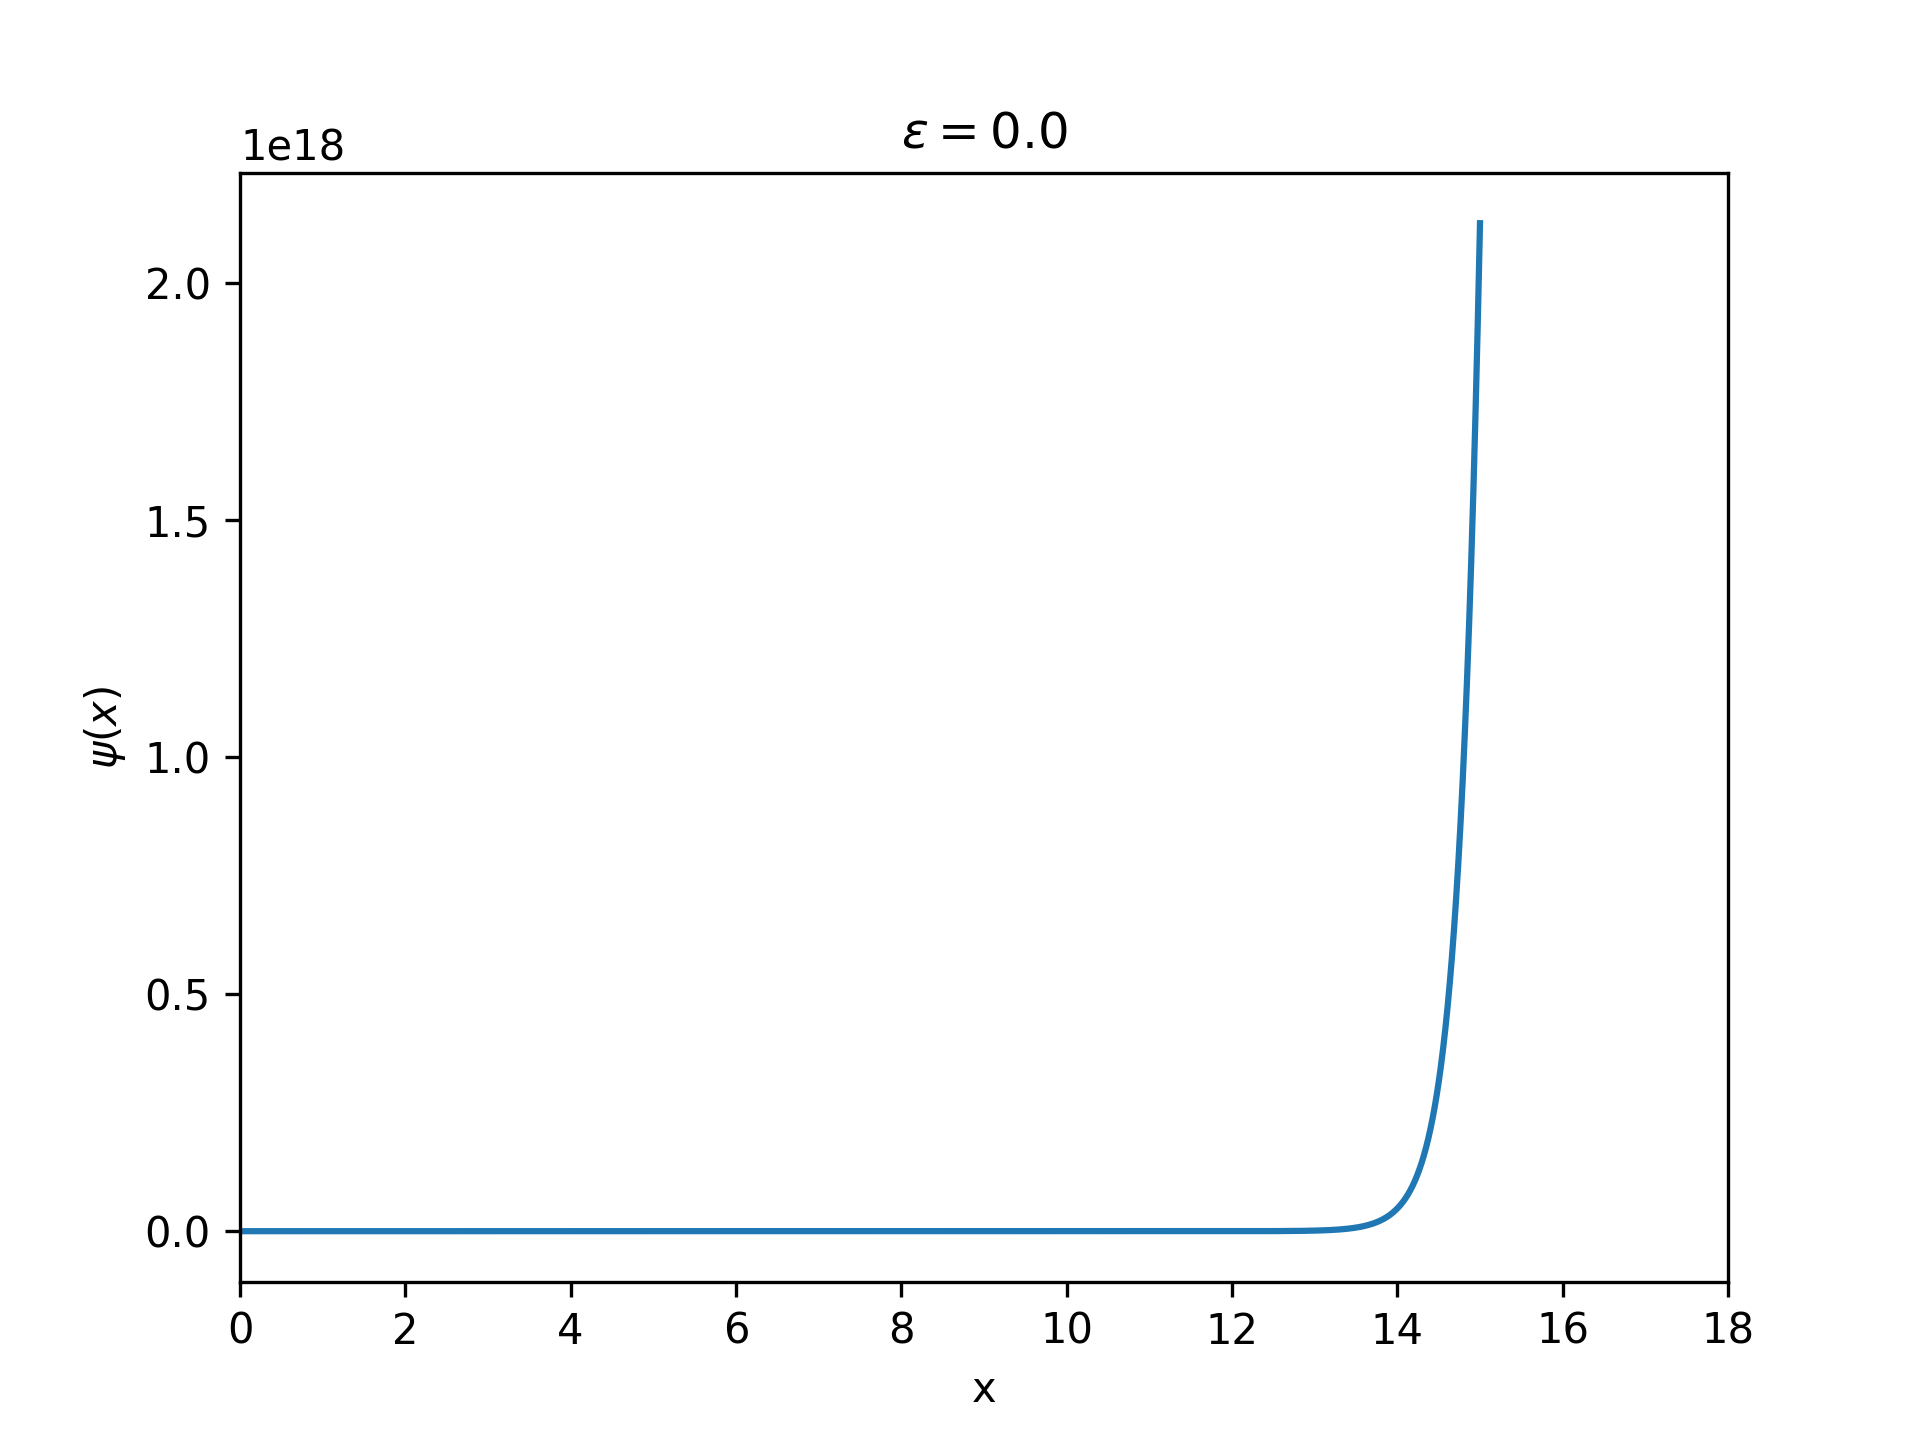
\includegraphics[width=.5\paperwidth]{plot_0_0.png}
    			\caption{positive asymptotic behaviour ($\epsilon = 0.0$)}
    		\end{figure}
    		
    		\begin{figure}[H]
    			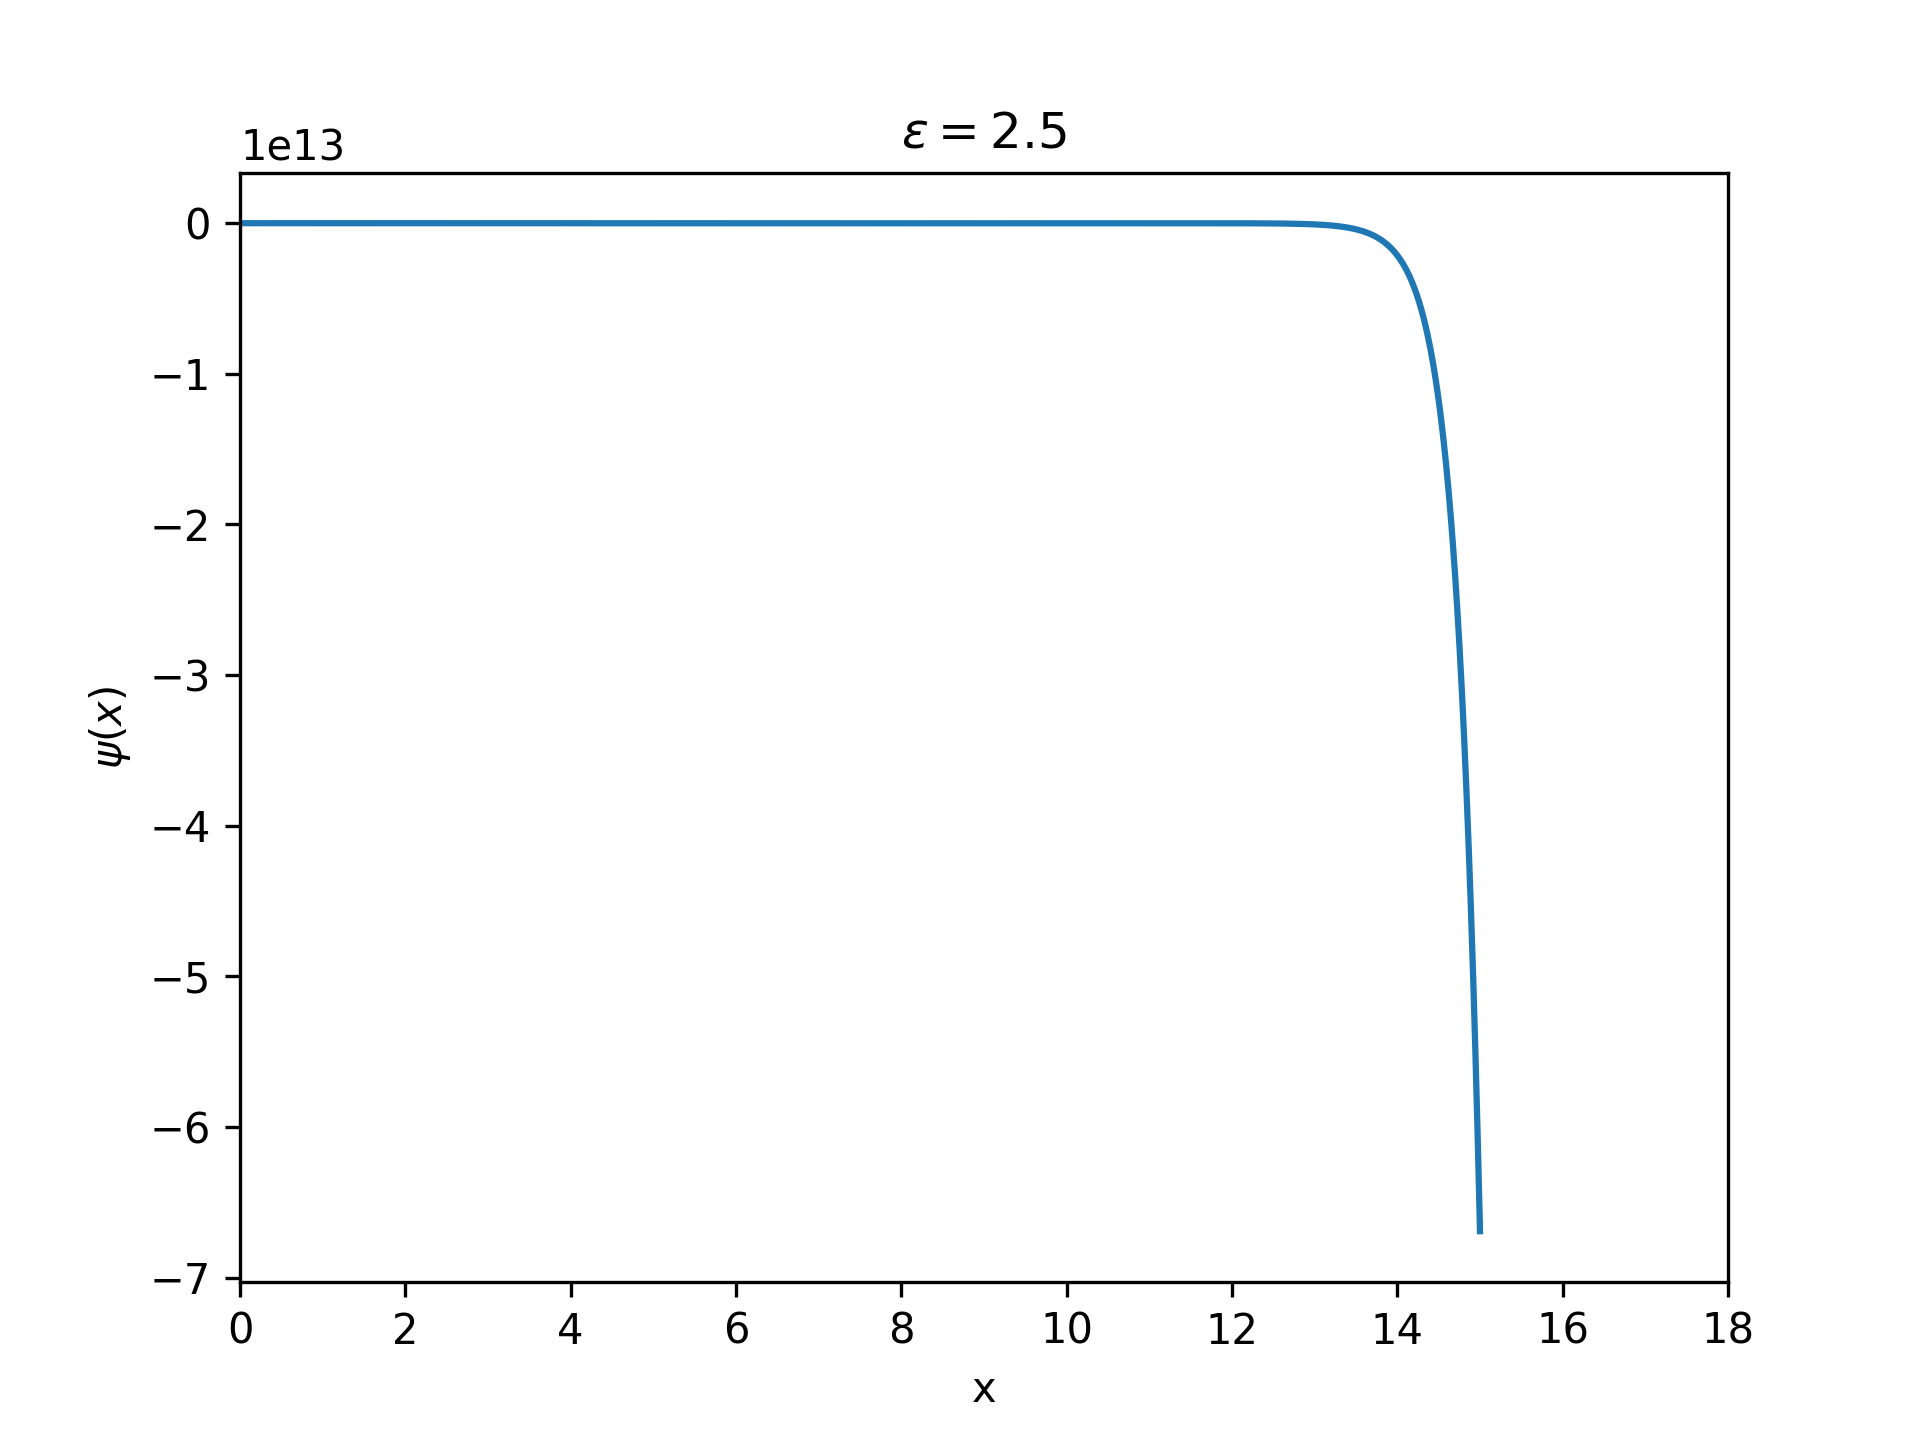
\includegraphics[width=.5\paperwidth]{plot_2_5.png}
    			\caption{negative asymptotic behaviour ($\epsilon = 2.5$)}
    		\end{figure}
    
    		
    %	\newpage
    		
    	\subsection*{2)}
    	To determine the eigenvalues $\epsilon_n$ we use the property of the sign 			change of the function $\Psi (x)$. We have modefied our code from before. 			You can choose a startenergy, a stepzise which you vary epsilon and how 			many sign changes you will search. The value of epsilon of a sign change 			will be printed. We start at $\epsilon = 0$ and chose our stepsize as the 			wanted decimals behind the comma.
    		
    	\begin{figure}[H]
        	\lstinputlisting[language=Python,
        		caption={Exercise04signChange.py},
        		lastline=63]{Exercise04signChange.py}        
    	\end{figure}
    	
    	The eigenvalues we found are: 
    	\begin{center}
    		$\epsilon_0 = 2.34$ \\
    		$\epsilon_1 = 4.09$ \\
    		$\epsilon_2 = 5.52$ \\
    	\end{center}
    	
    	\begin{figure}[H]
    			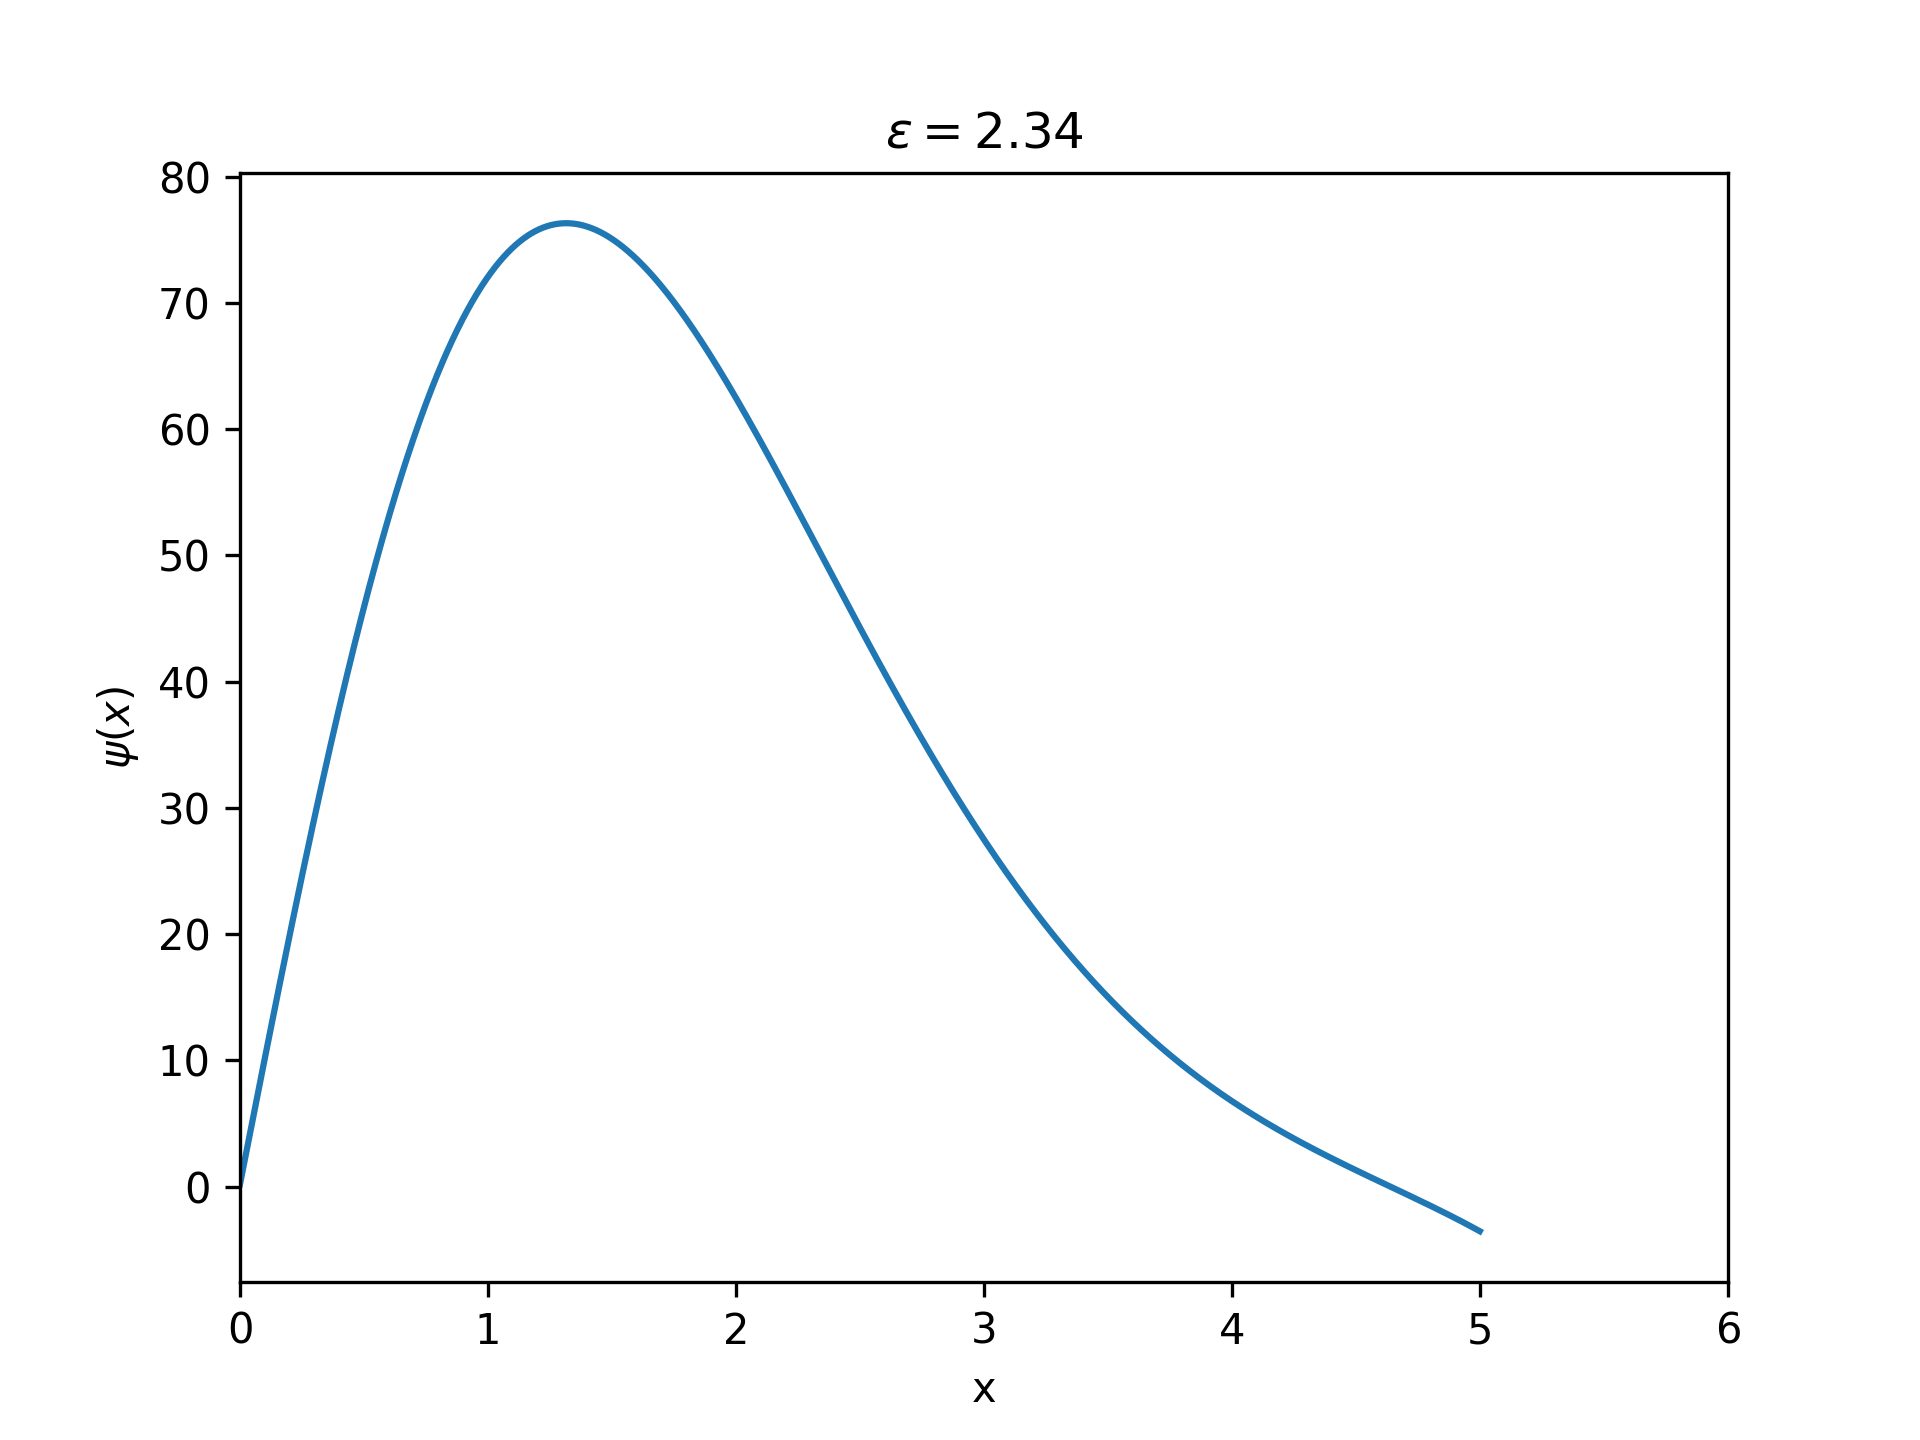
\includegraphics[width=.3\paperwidth]{plot_2_34.png}
    			\caption{eigenvalue ($\epsilon_0 = 2.34$)}
    	\end{figure}
    	\begin{figure}[H]
    			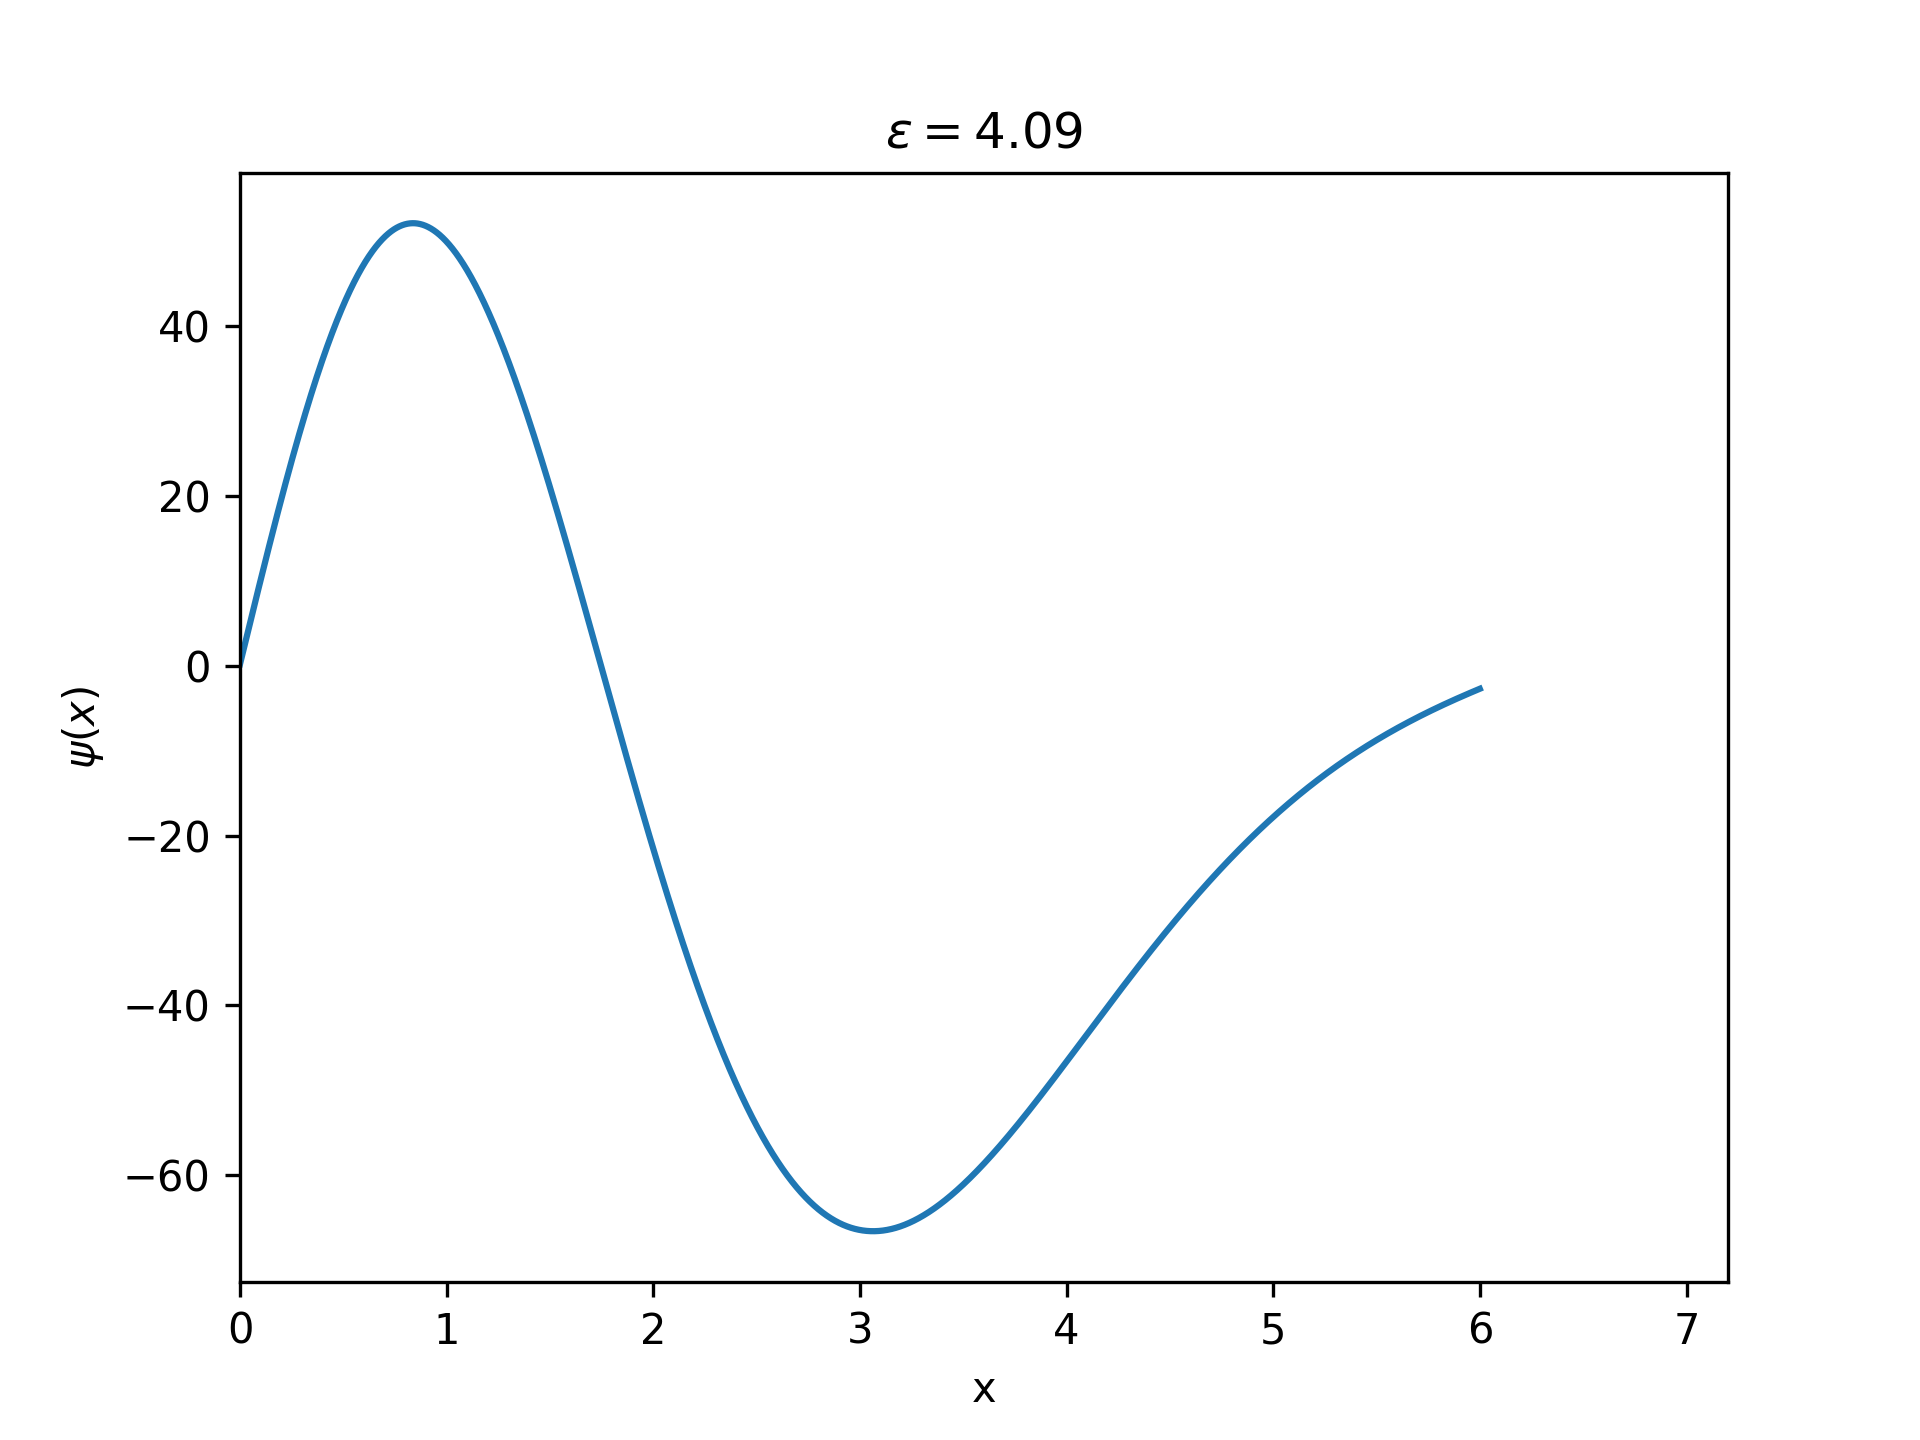
\includegraphics[width=.3\paperwidth]{plot_4_09.png}
    			\caption{eigenvalue ($\epsilon_0 = 4.09$)}
    	\end{figure}
    	\begin{figure}[H]
    			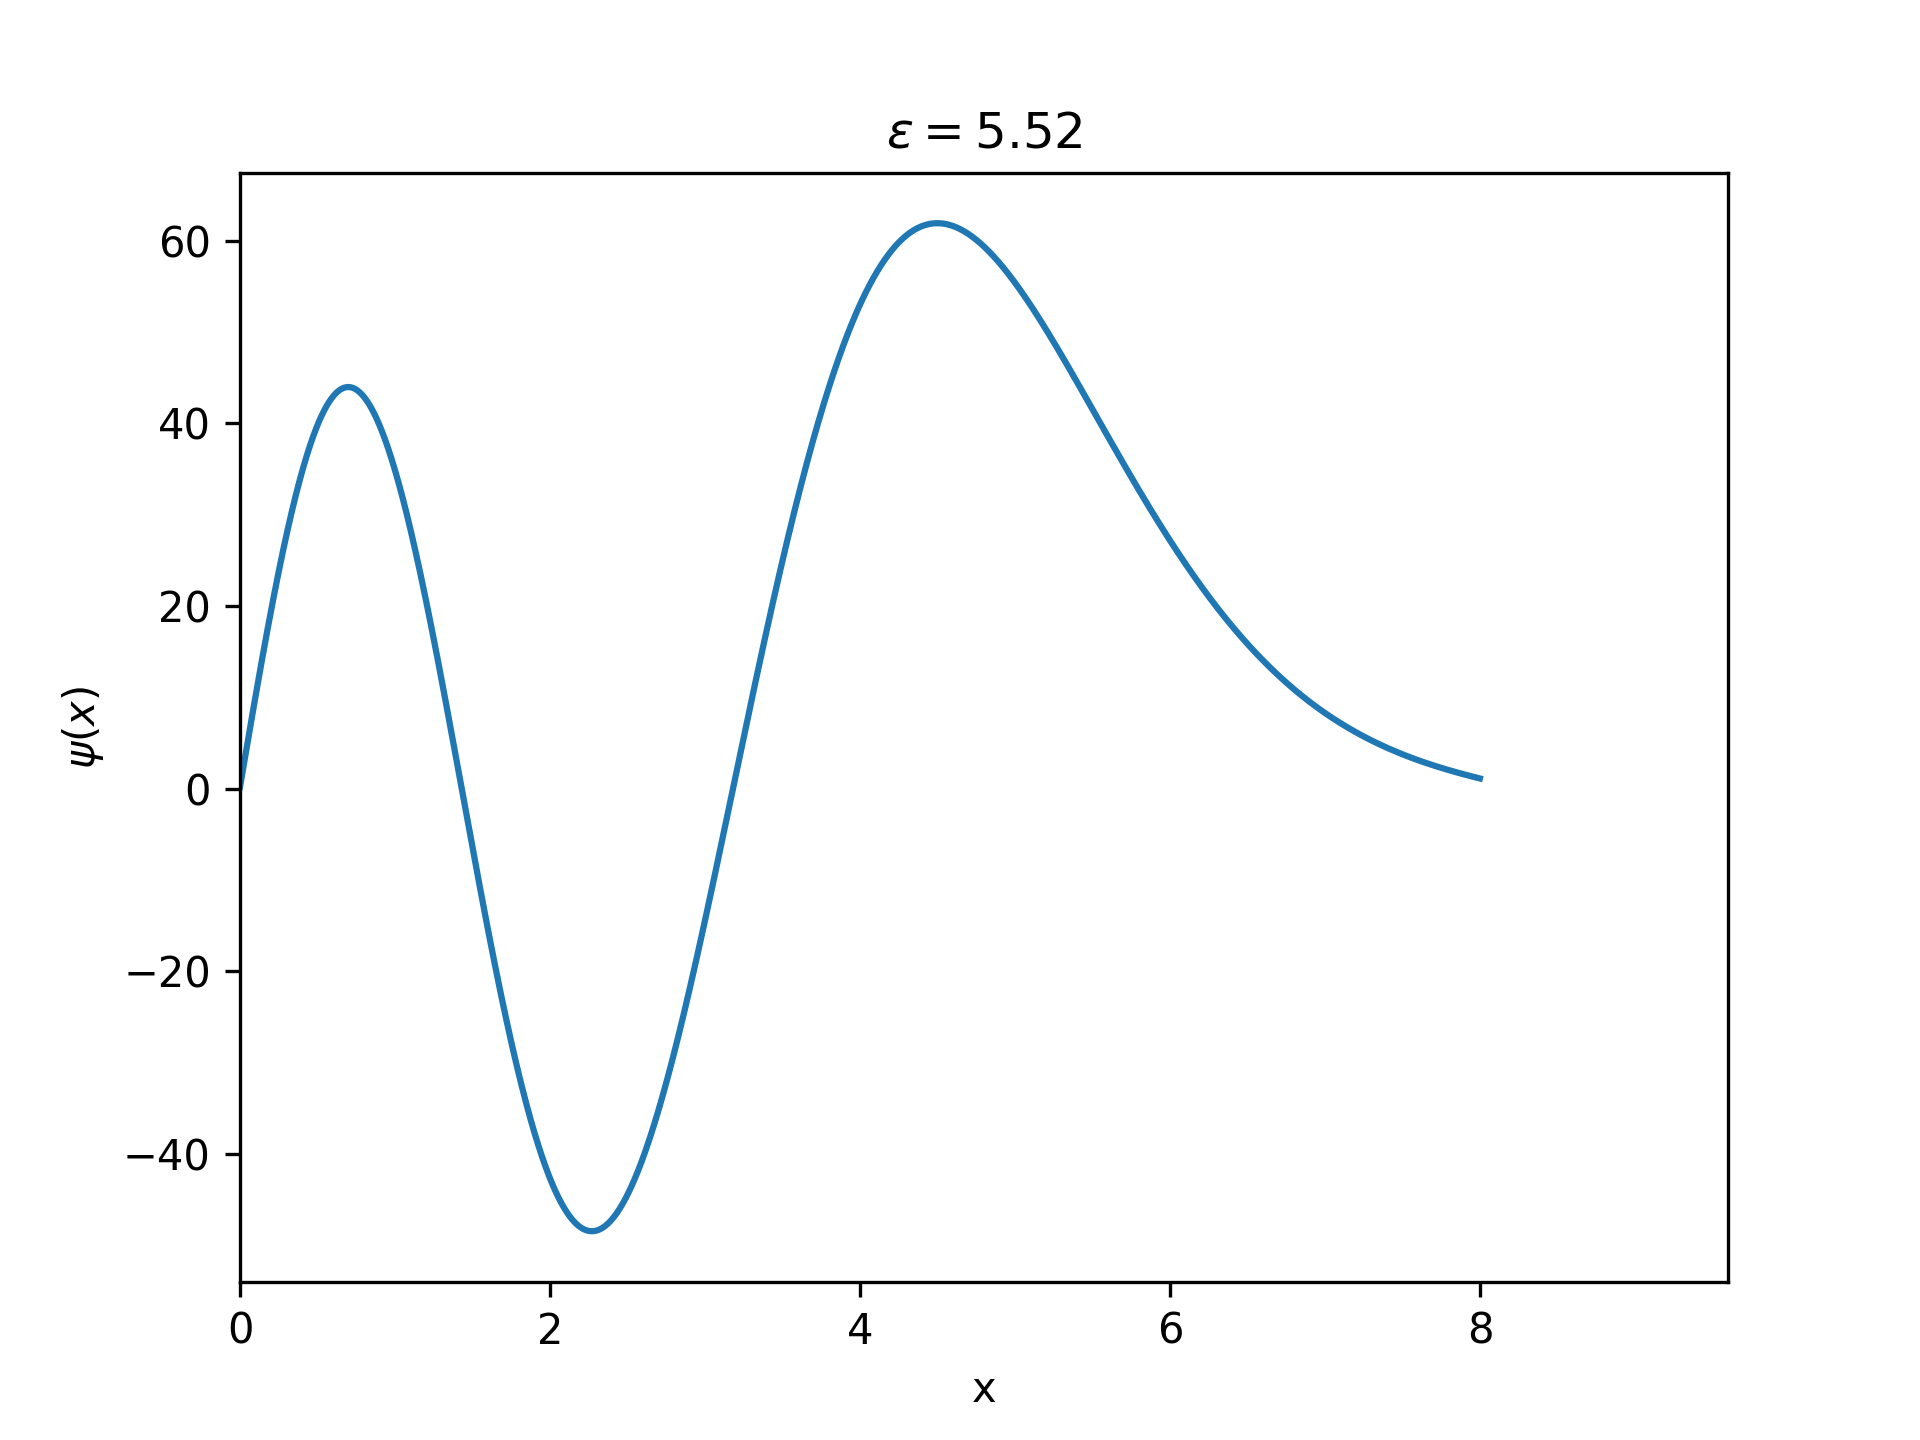
\includegraphics[width=.3\paperwidth]{plot_5_52.png}  		
    			\caption{eigenvalue ($\epsilon_0 = 5.52$)}
    	\end{figure}
    	
    		

\end{document}